\section{Measurements}
\label{sec:Measurements}

Data acquisitions of up to one million events have been taken at bias voltages ranging from $50$ to $450$~V for the mini sensors and from $50$ to $210$~V for the half size sensor.
In the case of the mini sensors, measurements at different angles of rotation around the $y$ axis, in the range between $-10$ and $20^\circ$, have also been taken, while only the nominal angle of $0^\circ$  has been considered in the case of the half size sensors.
For the mini sensors, the measurements have been repeated in two different sectors of the sensor, one at $y=0(2)$~mm, corresponding to the top edge of the sensor, where the pitch adapter is located, and another one at $y=10(18)$~mm, corresponding to the central region of the sensor.
For the half size sensor, seven sectors have been considered, as depicted in Fig. \ref{fig:F1}. This allows to inspect different regions of the pitch adapter and to check if the performances vary as a function of the hit position along the strips.

\begin{figure}[]
\centering
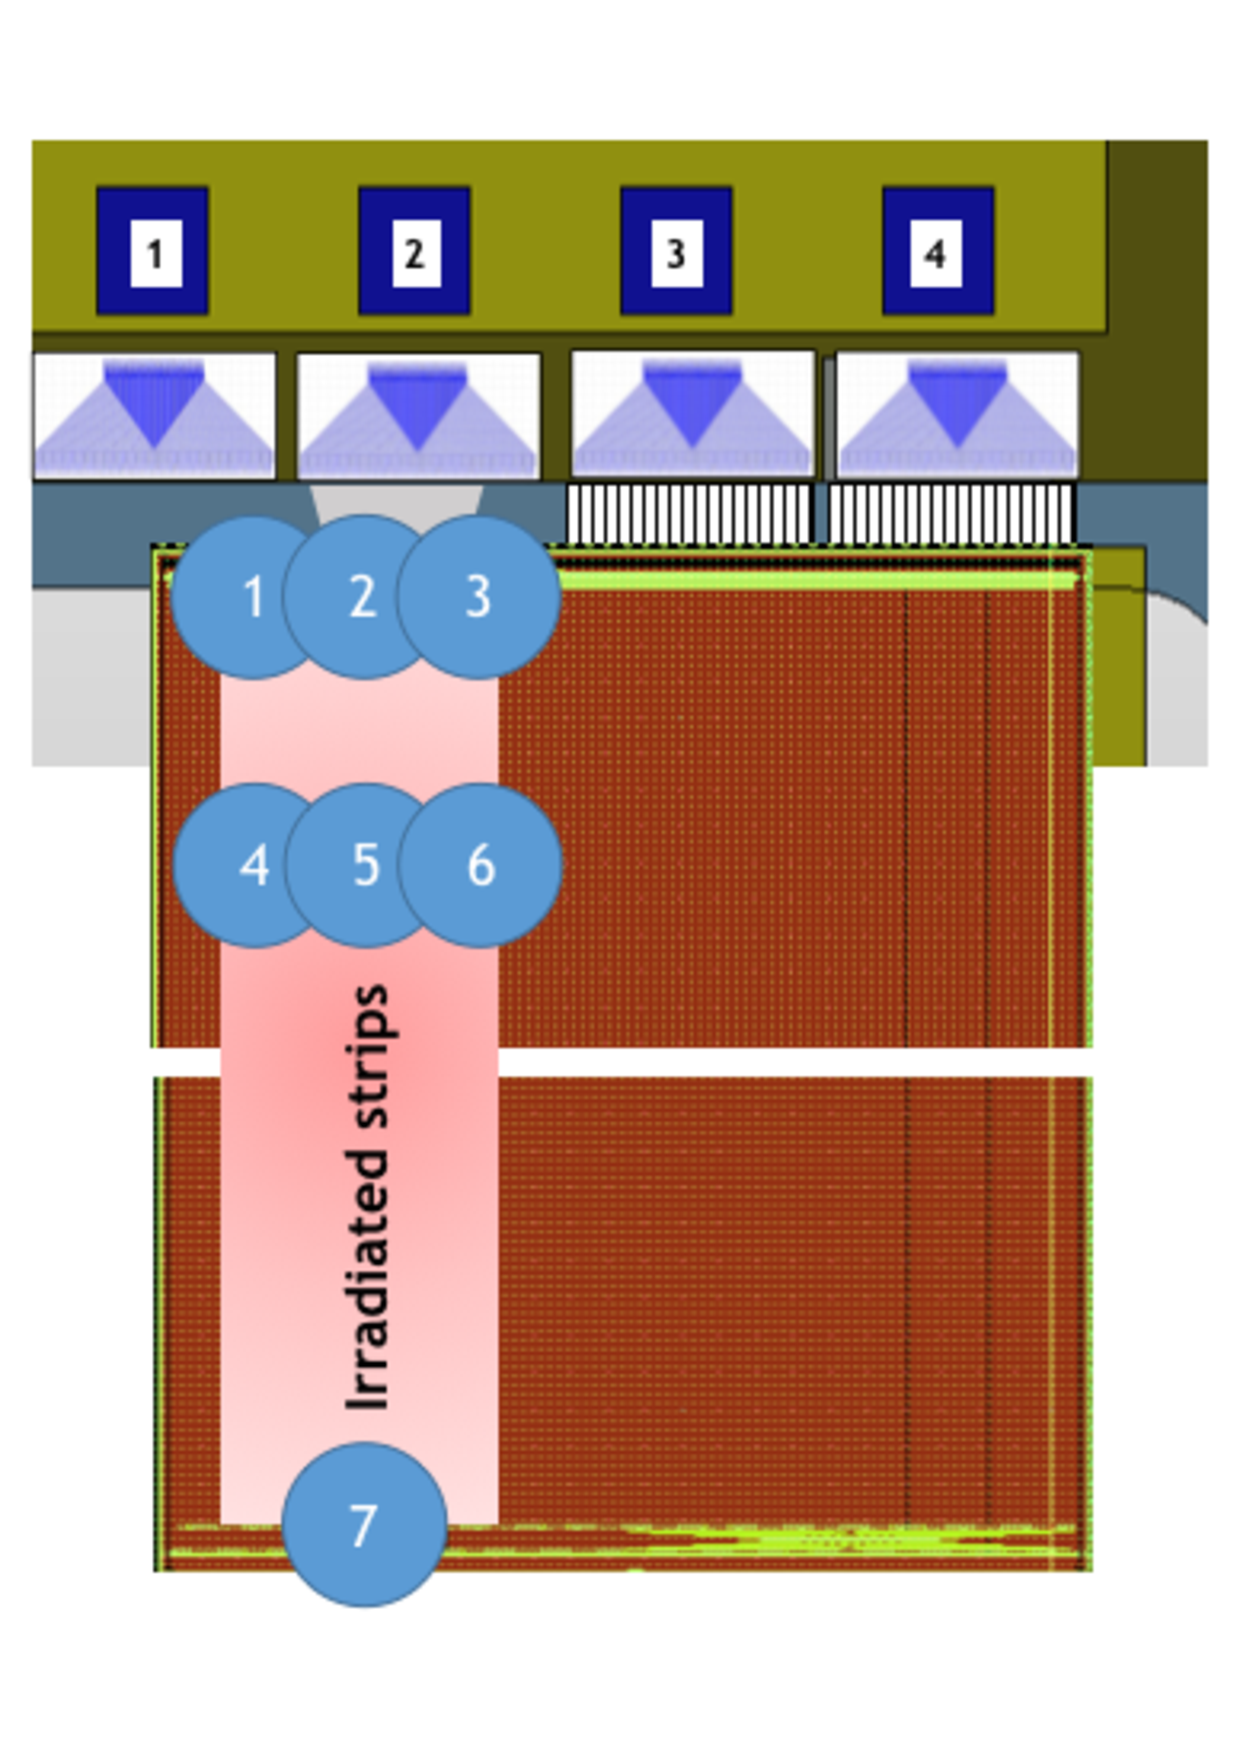
\includegraphics[width=0.4\textwidth]{figs/F1.pdf}
\caption[Layout of the half size p-in-n sensor.]{Layout of the full size p-in-n sensor.}
\label{fig:F1}
\end{figure}